\documentclass[a4paper]{scrreprt}
\usepackage{fancyhdr}
\pagestyle{fancy}
\usepackage[english]{babel}
\usepackage[utf8]{inputenc}
\usepackage{graphicx}
\usepackage{url}
\usepackage{textcomp}
\usepackage{amsmath}
\usepackage{lastpage}
\usepackage{pgf}
\usepackage{wrapfig}
\usepackage{fancyvrb}
\usepackage{appendix}
\usepackage{pdfpages}
\usepackage{xcolor}
\usepackage{hyperref}
\usepackage{placeins}

\hypersetup{
    colorlinks=true,
    linkcolor=blue,
    filecolor=black,      
    urlcolor=blue,
    citecolor=black,
}

% Create header and footer
\headheight 27pt
\pagestyle{fancyplain}
\lhead{\footnotesize{Datalagring, IV1351}}
\chead{\footnotesize{Task 3}}
\rhead{}
\lfoot{}
\cfoot{\thepage\ (\pageref{LastPage})}
\rfoot{}

% Create title page
\title{Task 3}
\subtitle{Datalagring, IV1351}
\author{Adrian Jonsson Sjödin \\ adriansj@kth.se}
\date{\today} 


\begin{document}

\maketitle

\tableofcontents %Generates the TOC

\chapter{Introduction}
The purpose of task 3 was to write OLAP queries towards the database created in task 2, and confirm that everything works as intended. The creation and reasoning behind 
the OLAP queries is what will be covered in this report.

\chapter{Method}
The DBMS used for the Sound Good Music School database is MySQL 8 and the queries was developed using a combination of DbGate and the CLI. The queries was tested manually 
by retrieving the data in question from the right tables and see if the query result matched was as expected.


\chapter{Result}
\label{sec:result}
The SQL scripts can be found here:
 \href{https://github.com/adrian-jonsson-sjoedin/IV1351-Datalagring/tree/main/project/SQL}{GitHub}.


\begin{figure}[h]
    \begin{center}
        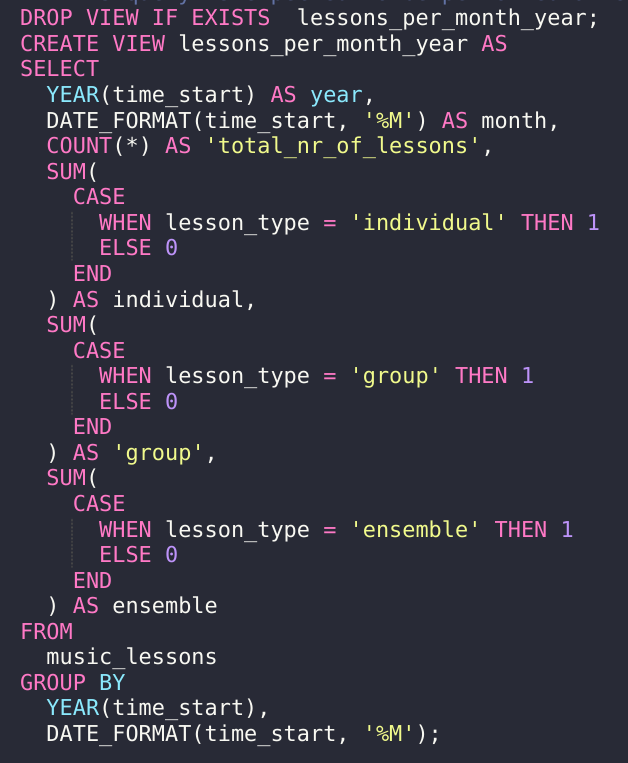
\includegraphics[width=0.70\textwidth]{../img/lessonsSQL.png} \\
        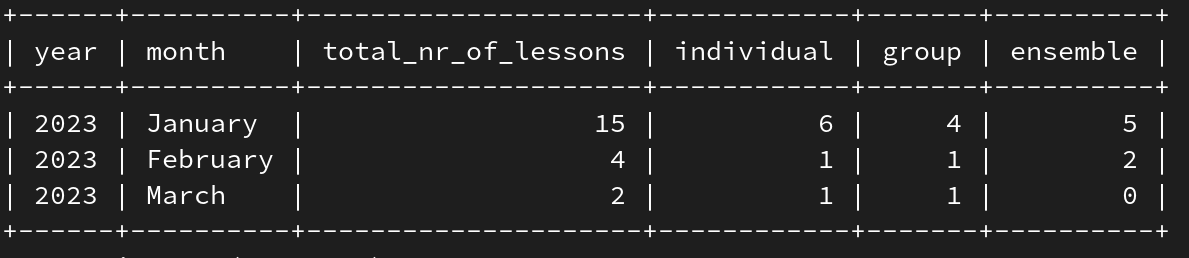
\includegraphics[width=0.70\textwidth]{../img/lessons.png}
        \caption{Total number of lessons per year and month for each lesson type}
        \label{fig:lessons}
    \end{center}
\end{figure}
\begin{figure}[h]
    \begin{center}
        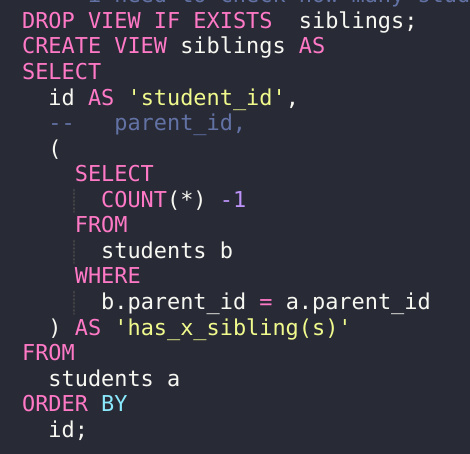
\includegraphics[width=0.49\textwidth]{../img/siblingsSQL.png} 
        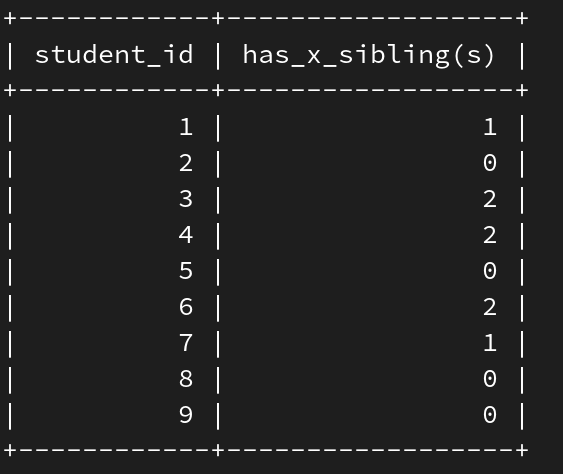
\includegraphics[width=0.49\textwidth]{../img/siblings.png}
        \caption{The number of siblings for each student}
        \label{fig:siblings}
    \end{center}
\end{figure}
\begin{figure}[h]
    \begin{center}
        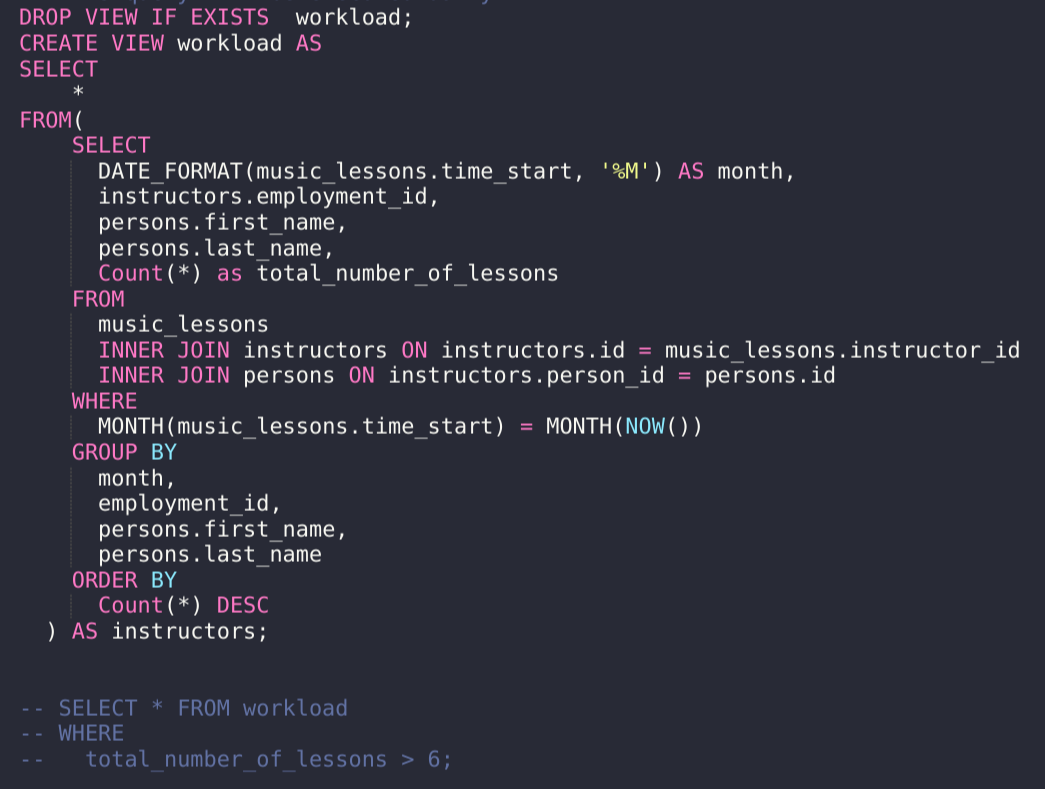
\includegraphics[width=0.76\textwidth]{../img/workloadSQL.png} \\
        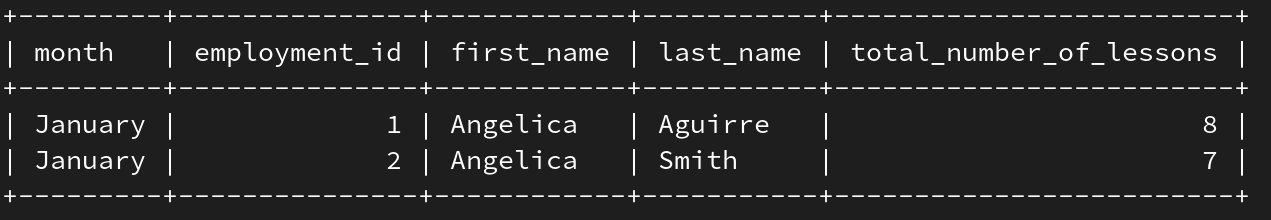
\includegraphics[width=0.76\textwidth]{../img/workload.png}
        \caption{List of all instructors that have more than a specific nr of lesson \\during the current month}
        \label{fig:workload}
    \end{center}
\end{figure}
\begin{figure}[h]
    \begin{center}
        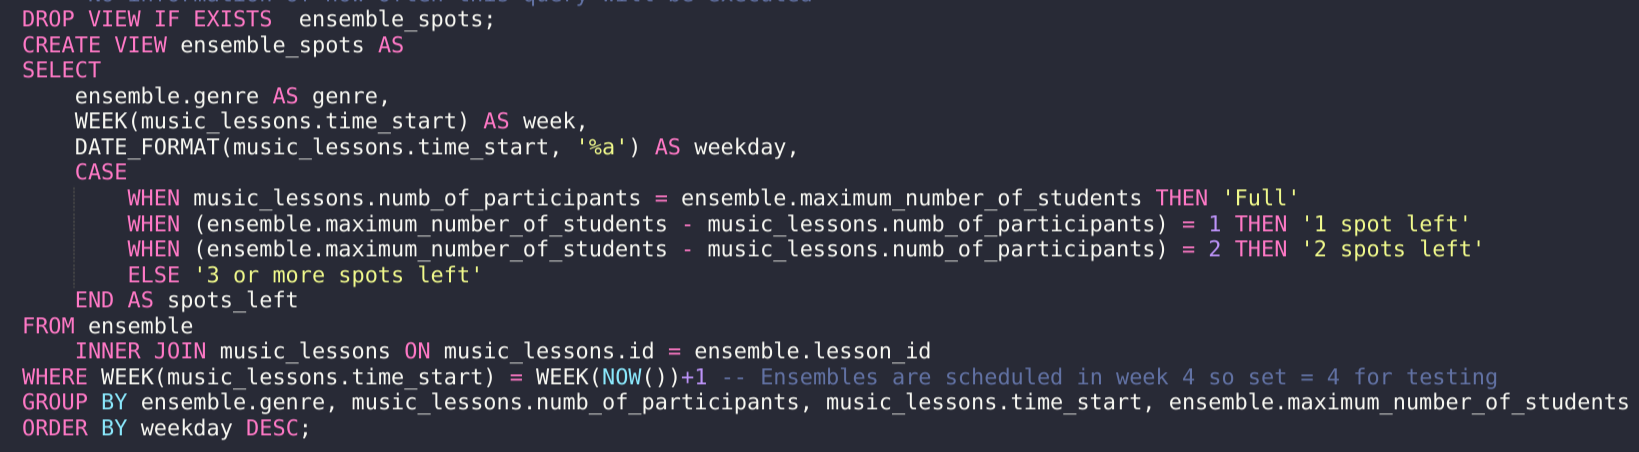
\includegraphics[width=\textwidth]{../img/ensembleSQL.png} \\
        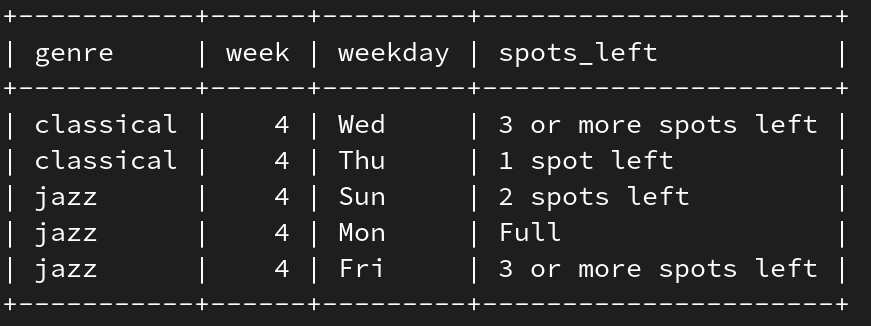
\includegraphics[width=\textwidth]{../img/ensemble_spots.png}
        \caption{List all ensembles held during the next week and how many spots are left, sorted by music genre and weekday}
        \label{fig:ensemble}
    \end{center}
\end{figure}
\begin{figure}[h]
    \begin{center}
        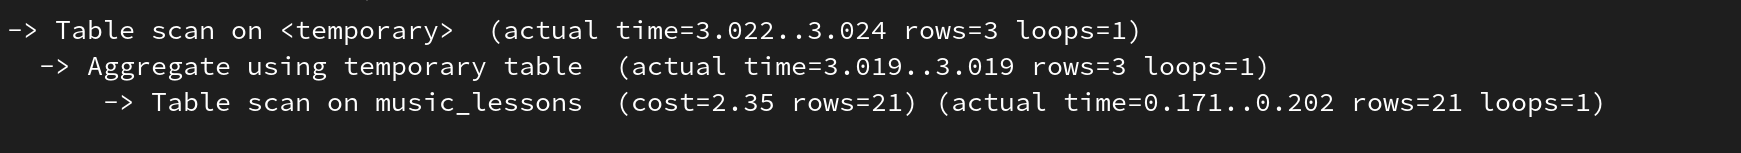
\includegraphics[width=\textwidth]{../img/explain_analyze_no_view_month_year.png} \\
        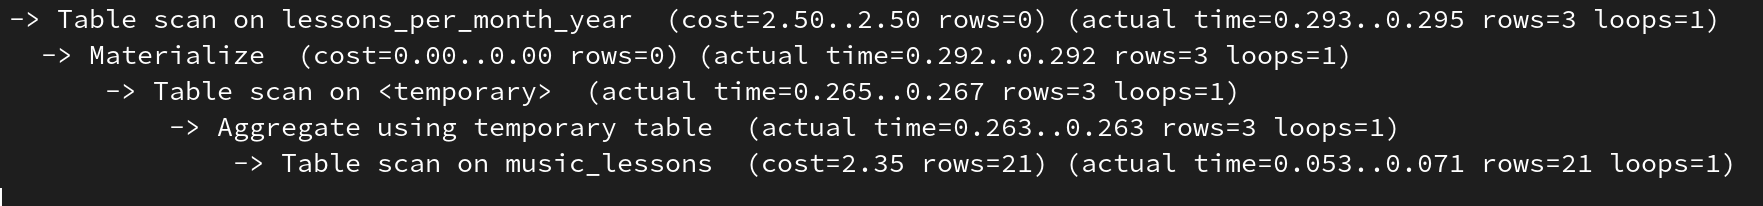
\includegraphics[width=\textwidth]{../img/explain_analyze_lessons_per_month_year.png}
        \caption{On top is the query from fig. \ref{fig:lessons} without storing it in a view while the bottom is the same query when stored in a view}
        \label{fig:explainLesson}
    \end{center}
\end{figure}
\begin{figure}[h]
    \begin{center}
        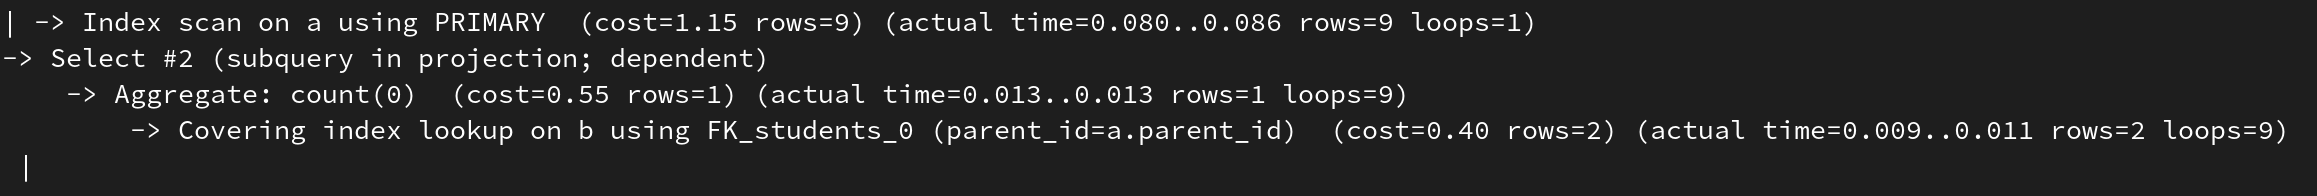
\includegraphics[width=\textwidth]{../img/explain_no_view_siblings.png} \\
        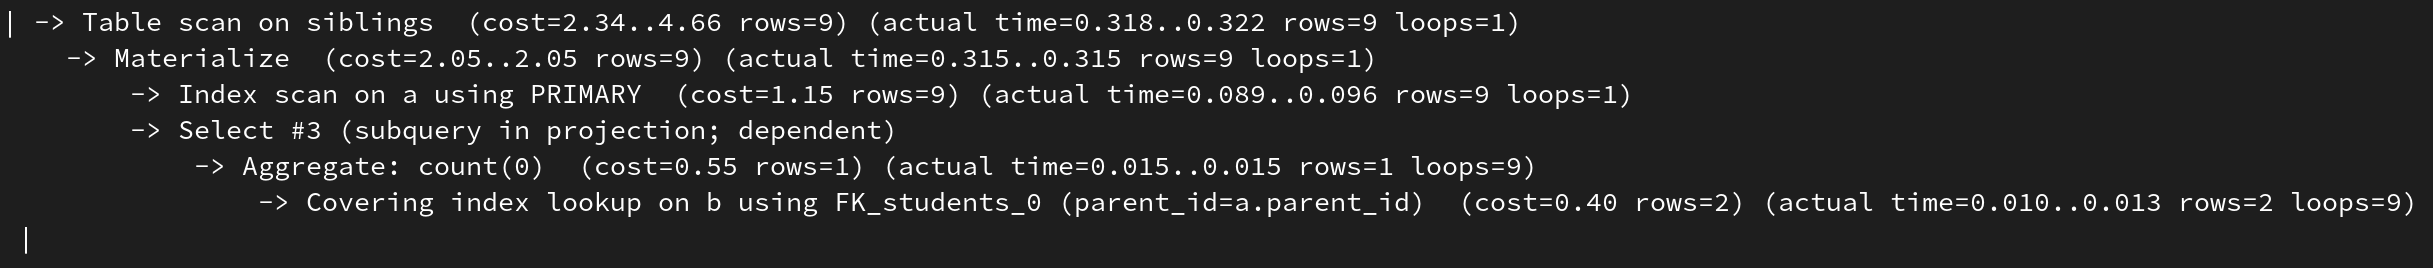
\includegraphics[width=\textwidth]{../img/explain_sibling.png}
        \caption{On top is the query from fig. \ref{fig:siblings} without storing it in a view while the bottom is the same query when stored in a view}
        \label{fig:explainSiblings}
    \end{center}
\end{figure}

The query seen in fig. \ref{fig:lessons} is the one that gives how many lectures we have per month and year and how many of each type. It is the easiest query out of 
the four and uses aggregate functions in combination with flow control functions.

The query seen in fig. \ref{fig:siblings} is the one that displays how many siblings each student have that is also enrolled at the school. This was the query that took
me the longest to write and has a correlated sub-query in the \textbf{SELECT} clause.

The third query is seen in fig. \ref{fig:workload} and is the one that list all instructors that have more than a specific number of lessons during the current month.
This query makes use of \textbf{INNER JOIN} to create a temporary table containing the data we wanted. 

Lastly we have the query seen in fig. \ref{fig:ensemble} which is the one that lists all available ensemble spots for the coming week. It utilizes a combination of flow
control functions to display available spots, and \textbf{INNER JOIN} to get the data from the two tables where the keys are matching.




\chapter{Discussion}
As can be seen from the queries in the Result section, all queries are stored as views. This is to make it easier to run them at a later date. All queries except the 
query seen in fig. \ref{fig:lessons} are stored in full. This was done because only that query had the requirement of being able to vary what was shown based of a 
requirement. The rest of them didn't have that condition and thus it would be easier to store the whole query as a view. 

The reason why I didn't use materialized view is simply because MySQL 8 (or earlier versions) doesn't seem to support it. If I could have used them then I would most 
likely have used them on query \ref{fig:lessons} and \ref{fig:siblings}. The first since I'm assuming the external application will create all lessons for multiple weeks
in advanced and thus not needing to update it very often. This would allow for a faster reading of data whenever it is needed, with the drawback of having to update the 
table whenever new lessons are added. But most likely that wouldn't be too often making it worthwhile turning it into a materialized view.

The same reasoning is behind why I would make query \ref{fig:siblings} into a materialized view. There will be a significant larger number of times I will read the table 
I get from that query as opposed to the number of times the materialized view would have to be updated. 

For the rest of the queries I think a view is the better choice since the columns containing the data we need to retrieve most likely will be updated often. For example 
the result from query \ref{fig:ensemble} will change whenever another students booking for an ensemble lessons is accepted, or they cancel their booking. And since the 
result will be displayed on the web page it needs to be up to date.

The database didn't need any permanent changes to make the queries. I did however make a temporary change by using DbGate to change the number of participants that had 
signed up for ensemble lessons larger. This so that I could test that query \ref{fig:ensemble} worked as intended. It was the easy solution for testing purpose since it
didn't require me to manually create more rows in the \textbf{bookings} table and match them with the corresponding music lesson (something that would be handled by 
the application that the administrative staff uses). 

As mentioned in the Result section, query \ref{fig:siblings} uses a correlated sub-query. It is possible I could get around this with more time and use some kind of 
\textbf{JOIN} operator instead, but currently I couldn't find a better solution. 

We see in fig. \ref{fig:explainLesson} that it took on average 0.202 ms to read all 21 rows in the \textbf{music\_lesson} table and that the aggregation took 3.019ms for
when the query was not stored as a view. And the outermost table scan took 3.024. Meaning the majority of the time was spent on the aggregation and the outermost table scan.
Giving us a total of about 6.23 ms. Looking at the result for the view we see that the reading of rows in the \textbf{music\_lesson} table was a bit faster and here 
taking 0.071 ms and the aggregation took only 0.263 ms. The outer table scan was also faster, clocking in at 0.267 ms. However we have two more costs in the view at 
0.292 ms and 0.295 ms, giving us a total of about 1.19 ms. This means that the view in this case is more than five times faster.

We don't get same result for the view and non view correlated sub-queries seen in fig \ref{fig:explainSiblings} however. There the view takes approximately 0.985 ms and
the non view takes approximately 0.302 ms, making the view more than three times slower in this case. 

\end{document}
